A typical statistical inference problem usually deals with estimation of unknown quantities based on some observed information. Due to their many desirable qualities like ability to provide uncertainty around the estimations, seamless incorporation of new information to the model and elimination, Bayesian methodology has considerable advantage over other approaches to data analysis and statistical inference. In this section we briefly review the bayesian inference and then explore inference problem from a non parametric perspective. Section 2.2 further provides a introduction to Gaussian Processes as a bayesian non parametric method and finally a short overview of sparse approximation technique is provided in section 2.2.3

\subsection{Bayesian Inference}

Bayesian methods approach the solution of inference problem from a probabilistic perspective by setting up a model that constitutes our assumptions and knowledge about all relevant observed as well as unobserved quantities as probabilistic statements. 
The complete inference process then consists of three steps, First formulation of initial knowledge about the model and its constituents in terms of prior and joint distribution. Bayes’ theorem is then used to figure out the posterior - conditional probability distribution of unobserved quantities given the observed ones. This posterior distribution is considered to be the underlying distribution from which all unobserved quantities were generated in the past and will continue to do so in future. Finally, a formal validation step can be performed to determine model’s ability to explain the observations and thereby its correctness[BDA, A gelmen].
Thus in a generic Bayesian analysis process, parameters describe the particular data generating model we believe the observations arose from and the inference process becomes about finding the possible values of parameters that could generate the given observations:
\begin{equation}
\scriptstyle
P(parameters | observation, model) =  P(observations | parameters, model) P(parameters,model)
\end{equation}

Here the first term at RHS tells us the probability of seeing those observations given a particular set of parameters i.e. likelihood and the second term incorporates our belief about those parameter values before seeing the observations, i.e. prior.
Once the posterior is identified, that means models and its parameters have been recognized one could either generate or predict new data:

\begin{equation}
\scriptstyle
    P(x| parameters, observation,model) = \integration P(x | parameters , observation, model) P(parameters |observation, model)
    \label{eqn:general_margin}
\end{equation}

\subsubsection{Parametric and Non Parametric Models}

Based on the specific problem at hand, we usually make certain assumptions about the model. These salient properties of model are included in the inference process as the model parameters. For example, its common to assume sampling distribution of a continuous quantity to be normal. In that case mean and variance would be termed as model parameters. Similarly, number of clusters would be a parameter in case of a mixture model. The specific parameters value then can be used describe that particular model. Once the value of these parameters are known, the model is said to be identified, i.e. complete knowledge about observed data and its generating process is transferred in the parameters from observations. From the perspective of equation \ref{eqn:general_margin}, 
 $$P(x| parameters, data, model) =  P(x| parameters, model)$$
Or in other words, parameters have extracted ‘everything there was to know about data releavent to future predicitons’ [http://mlg.eng.cam.ac.uk/pub/pdf/Gha12.pdf.] 

However, this requirement of making initial assumption about parameters means for parametric mdoels underlying distribution is restricted to be in the same category as the other models with similar parameterization. [O’Hagan book] This restriction as we will see later makes these models inflexible and of limited capacity. 

Conversely, in cases where we want to make no assumptions to restrict the model we stipulate a generic model with no fixed number of parameters and call them non-parametric models. A non parametric regression model for example would not consider any specific function form but just a collection of functions one of which might have generated the observations. 

Since the model is considered to be the process that generated the observational data during data analysis, another way to look at the distinction between parametric and non parametric is by considering our model to be a subset of the set of all data generating processes defined in a parameter space that is indexed by a vector of model parameters. A parametric model then will have a finite length parameter vector identifying a subset of data generating process while non parametric model will have infinite number of parameters representing unrestricted amount of models that can be considered (Figure \ref{fig:generic_function_space}). 
\begin{figure}
    \centering
    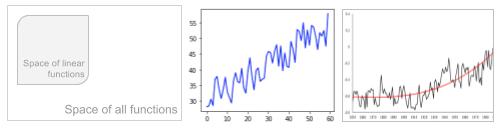
\includegraphics[scale=0.75]{thesis/images/function_spaces.png}
    \caption{Left: Illustration of function spaces and linear spaces with in it, Middle: A linear trend, Right: Non Linear trend}
    \label{fig:generic_function_space}
\end{figure}
Apart from possibility to consider a richer set of models by making minimal assumptions, non parametric models also provide a coherent way of model criticism and prior selection. In Bayesian analysis, the prior beliefs used to derive posterior must represent the actual state of knowledge without the knowledge of observations. Thus, the model selection approach to alleviate prior uncertainty by first using multiple priors and then selecting one of them based on the most convincing posterior results (after looking at the observation) is not considered coherent, specially in Bayesian paradigms where appropriately used methods should not overfit any ways [http://www.gatsby.ucl.ac.uk/~edward/pub/occam.pdf, Mackay 91] A non parametric approach on the other hand goes around models selection issue due to its ability to specify unrestricted forms can be used to accommodate the uncertainty around priors [Bayesian Non Paramterics book].

This problem of choosing a model’s parameters beforehand or model selection has prime importance in machine learning arena. Improper model selection significantly impacts a model’s performance through generating an over or under fitted model. Moreover, some use cases where identification of underlying structure of data is important like hidden Markov models, mixture models etc., might require one to supply the parameters even before the inference process has begun. Usual solution to these model selection issues is to perform cross validation [reference missing]. However, depending upon the situation it might either be inefficient to compare all the possible models or simply incoherent from Bayesian perspective as explained in the previous paragraph to reuse data multiple times. Bayesian Nonparametric methods gets around this problem by adapting the complexity of model based on available data, [Baysian nonparametric methods paper] i.e allowing for gradually more complex model as the amount of data grows. For example, a traditional mixture model requires number of clusters to be fixed before hand while non parametric approach would be able to infer even the number of clusters from the data and allows it to increase as it encounters new data. [Chinese buffet process, drichlet process article]

\subsubsection{Non parametric models}

In most machine learning application our objective is to find a ‘pattern’ that can be used to explain observed data. In most cases a function can be used to represent this pattern and thus our objective becomes to search for the function among many possible functions that best explains the data. However, we might reduce the search space by making some common sense assumptions. For example, to find the function that explain clearly linear data in Figure \ref{fig:generic_function_space}(middle) one might want to search within smooth linear function spaces while in case of Figure \ref{fig:generic_function_space}(right) we would like to relax the linear constraint and search among all possible smooth functions.  As can be observed, this is analogous to putting prior over parameters in Bayesian analysis but now parameter space represents all possible functions and prior encapsulates our initial guess about the space where our viable solution should exist. 

It is clear form above discussion that Bayesian nonparametric model requires us to put probability distribution over these functions (infinite dimensional objects). Beginning from Fergusson’s work on Drichlet’s processes [T. Fergusson 1973] various strategies have been recommended to build these models. [Neil, 2005] for example recommends starting from a parametric model and then take infinite limit of it. Due to their propensity to work with infinite dimensional objects, a lot of work in this field have been done under stochastic process analysis. Historically Drichlet process  and Gaussian processes have dominated the nonparametric models. Drichlet’s process is sued to put distribution over distributions and hence has been primarily used in relation to density estimation or topic modelling related problem[Reference to Ferguson paper and other DP papers]. Gaussian Processes are another famous tool set that have been used extensively to solve Bayesian nonparametric problems where funcitons are to be estimated, i.e. putting distributions over functions. Next section explores Gaussian processes in more detail.







